\section{Illustrative Extension: Clawbacks and Policy Design}\label{sec:extensions}

Sections \ref{sec:subsidy} and \ref{sec:decentralized} contain the paper's core analytical contribution. This section is deliberately illustrative: it introduces a second instrument only to show, in reduced form, how policy design could target the composition margin created by buyout exit. A uniform entry subsidy affects only the extensive margin. It cannot alter private project choice and therefore cannot correct that distortion on its own.

\subsection{A buyout-contingent clawback}

We model the clawback as a reduced-form tax on the entrepreneur's merger-related continuation payoff. The goal is to isolate the composition effect of reducing the entrepreneur's private reward from sell-out-oriented innovation while holding fixed the merger technology and product-market consequences of acquisition.

\begin{assumption}\label{ass:clawback}
The clawback redistributes merger-related gains away from the entrepreneur without changing the joint surplus from attempting a merger, the merger technology itself, or the realized product-market outcome conditional on approval.
\end{assumption}
This is a maintained invariance assumption used to keep the extension transparent; it is not intended as a complete institutional description of all clawback arrangements.

Under Assumption \ref{ass:clawback}, the merger-attempt condition remains
\begin{equation}\label{eq:attemptconditionrho}
    q\Delta_j \ge k,
\end{equation}
so the attempt indicator is unchanged:
\begin{equation}
    a_j(q)=\mathbf{1}\{q\Delta_j \ge k\}.
\end{equation}
Because realized product-market outcomes and merger feasibility are unchanged, the welfare objects \(B_j^L(q)\) and \(B_j^N(q)\) remain those defined earlier. The clawback operates only through private continuation values and the induced changes in effort, entry, and project choice.

If the entrepreneur must remit a fraction \(\rho \in [0,1)\) of merger-related continuation gains, then conditional on success and project choice \(j\), private continuation value becomes
\begin{equation}\label{eq:Rtilde}
    \widetilde R_j(q,\rho)
    =
    \pi_E^D(j)
    +
    (1-\rho)\beta [q\Delta_j-k]_+.
\end{equation}
Under the corresponding interiority condition,
\begin{equation}
    \widetilde x_j^*(q,\rho)=\widetilde R_j(q,\rho),
    \qquad
    \widetilde U_j(f;s,q,\rho)=s-f+\frac{\widetilde R_j(q,\rho)^2}{2}.
\end{equation}
Define
\begin{equation}
    \widetilde A_j(q,\rho)\equiv \frac{\widetilde R_j(q,\rho)^2}{2},
    \qquad
    \widetilde c_j(s,q,\rho)\equiv s+\widetilde A_j(q,\rho).
\end{equation}
Then the mass of entrants under project \(j\) is \(\widetilde n_j(s,q,\rho)=\widetilde c_j(s,q,\rho)\).

\begin{proposition}\label{prop:clawbackthreshold}
Suppose Assumptions \ref{ass:types} and \ref{ass:singlecross} hold, and consider values of \(q\) such that both project types are merger-feasible. Then there exists a unique project-switching threshold
\begin{equation}\label{eq:qhatrho}
    \hat q(\rho)
    =
    \frac{
        \pi_E^D(I)-\pi_E^D(B)
    }{
        (1-\rho)\beta(\Delta_B-\Delta_I)
    }.
\end{equation}
The entrepreneur chooses the buyout-oriented project if and only if \(q>\hat q(\rho)\), and
\begin{equation}\label{eq:dqhatdrho}
    \frac{\partial \hat q(\rho)}{\partial \rho}
    =
    \frac{\hat q(\rho)}{1-\rho}
    >0.
\end{equation}
\end{proposition}

A higher clawback therefore makes buyout-oriented innovation less attractive by shifting the switching threshold to the right. For any fixed approval probability \(q\), the minimal clawback required to restore the independence-oriented project is
\begin{equation}\label{eq:rhobar}
    \bar \rho(q)
    \equiv
    \max\left\{
        0,\;
        1-
        \frac{
            \pi_E^D(I)-\pi_E^D(B)
        }{
            \beta q(\Delta_B-\Delta_I)
        }
    \right\},
\end{equation}
provided both projects are merger-feasible.

Figure \ref{fig:clawback_threshold_calibrated} illustrates this threshold effect under the benchmark calibration.

\begin{figure}[t]
\centering
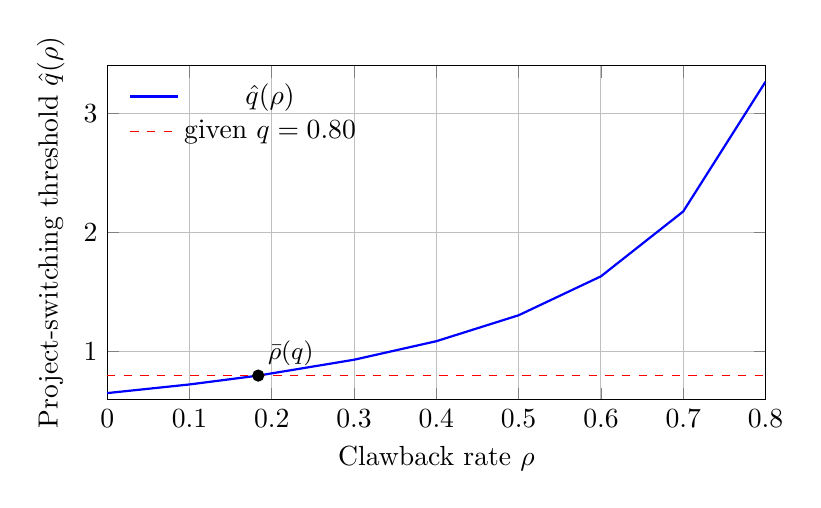
\begin{tikzpicture}
\begin{axis}[
    width=0.82\textwidth,
    height=0.48\textwidth,
    xmin=0, xmax=0.8,
    ymin=0.60, ymax=3.4,
    xlabel={Clawback rate \(\rho\)},
    ylabel={Project-switching threshold \(\hat q(\rho)\)},
    legend style={draw=none, fill=none, at={(0.02,0.98)}, anchor=north west},
    ymajorgrids=true,
    xmajorgrids=true
]

\addplot[thick, blue] coordinates {
(0,0.6531405543)
(0.1,0.7257117270)
(0.1835743071,0.8000000000)
(0.3,0.9330579347)
(0.4,1.0885675905)
(0.5,1.3062811086)
(0.6,1.6328513858)
(0.7,2.1771351810)
(0.8,3.2657027715)
};
\addlegendentry{\(\hat q(\rho)\)}

\addplot[red, dashed] coordinates {(0,0.80) (0.8,0.80)};
\addlegendentry{given \(q=0.80\)}

\addplot[only marks, mark=*, mark size=2pt] coordinates {(0.1835743071,0.80)};
\node[anchor=south west] at (axis cs:0.1836,0.80) {\small \(\bar\rho(q)\)};

\end{axis}
\end{tikzpicture}
\caption{Illustrative effect of a buyout-contingent clawback on the project-switching threshold under the calibration reported in the text. Since \(\hat q(\rho)\) increases in \(\rho\), a higher clawback makes buyout-oriented innovation less attractive for any given approval probability \(q\).}
\label{fig:clawback_threshold_calibrated}
\end{figure}

\subsection{Subsidy formulas under a clawback}

Because the clawback changes private continuation values but not welfare incidence for a given realized outcome, the local planner's type-\(j\) welfare becomes
\begin{equation}\label{eq:WtildeL}
    \widetilde W_j^L(s,q,\rho)
    =
    \widetilde c_j(s,q,\rho)
    \left(
        \widetilde R_j(q,\rho)B_j^L(q)
        -
        \widetilde A_j(q,\rho)
        -
        \tau s
    \right)
    -
    \frac{\widetilde c_j(s,q,\rho)^2}{2},
\end{equation}
with optimal subsidy
\begin{equation}\label{eq:stildeclaw}
    \widetilde s_j^{L*}(q,\rho)
    =
    \max\left\{
        0,\;
        \frac{
            \widetilde R_j(q,\rho)B_j^L(q)
            -
            \frac{\tau+2}{2}\widetilde R_j(q,\rho)^2
        }{2\tau+1}
    \right\}.
\end{equation}
Similarly,
\begin{equation}\label{eq:stildeclawn}
    \widetilde s_j^{N*}(q,\rho)
    =
    \max\left\{
        0,\;
        \frac{
            \widetilde R_j(q,\rho)B_j^N(q)
            -
            \frac{\tau+2}{2}\widetilde R_j(q,\rho)^2
        }{2\tau+1}
    \right\}.
\end{equation}
Whenever both are interior,
\begin{equation}\label{eq:wedgeclawback}
    \widetilde s_j^{L*}(q,\rho)-\widetilde s_j^{N*}(q,\rho)
    =
    \frac{
        \widetilde R_j(q,\rho)\bigl(B_j^L(q)-B_j^N(q)\bigr)
    }{2\tau+1}.
\end{equation}
Thus the clawback rescales the magnitude of the local--national wedge for a given project type, while potentially changing the equilibrium wedge indirectly through project switching.

\subsection{Illustrative joint design with merger policy}

Let \(\theta\) denote a policy shifter of \(q\), with antitrust toughness as one interpretation:
\begin{equation}
    q=q(\theta),
    \qquad
    q'(\theta)<0.
\end{equation}
Under a clawback, project \(B\) is privately chosen whenever \(q(\theta)>\hat q(\rho)\). Hence the set of policy pairs \((\theta,\rho)\) that leave the entrepreneur indifferent between projects satisfies
\begin{equation}\label{eq:implementationlocus}
    q(\theta)=\hat q(\rho).
\end{equation}

\begin{proposition}\label{prop:instrumentsubstitution}
Suppose \(q'(\theta)<0\), and consider the locus of policy pairs \((\theta,\rho)\) satisfying \eqref{eq:implementationlocus}. Then:
\begin{enumerate}
    \item A higher clawback rate \(\rho\) permits a lower antitrust toughness \(\theta\) while keeping project choice unchanged.
    \item The independence-oriented project can be implemented by stricter merger policy, a stronger clawback, or a combination of the two.
    \item Along the implementation locus,
    \begin{equation}\label{eq:dthetadrho}
        \frac{d\theta}{d\rho}
        =
        \frac{\hat q'(\rho)}{q'(\theta)}
        <0.
    \end{equation}
\end{enumerate}
\end{proposition}

Within this illustrative extension, clawbacks and merger policy are therefore substitute instruments for the composition margin. A stronger clawback reduces private sell-out incentives directly, whereas stricter merger policy does so indirectly by lowering the probability of approved acquisition.

\subsection{Illustrative policy-design implications}

The extension reinforces a simple policy-design lesson. Uniform entry subsidies are useful for the extensive margin but poorly suited to environments in which the main concern is the \emph{type} of startups being created. A buyout-contingent clawback adds a second instrument that directly targets composition. In the present framework,
\begin{itemize}
    \item the subsidy \(s\) governs how many entrepreneurs enter,
    \item the clawback \(\rho\) governs how attractive buyout-oriented innovation is relative to independence-oriented innovation, and
    \item merger policy \(q\) or \(\theta\) governs the overall exit environment.
\end{itemize}
This separation of instruments is especially relevant when local and national planners value acquisition-oriented entrepreneurship differently, but the discussion here should be read as a proof-of-concept extension rather than as the paper's central institutional result.
